 \documentclass[book.tex]{subfiles}
\begin{document}
My personal introduction to computer gaming began in 1985, when my parents bought an MSX-1 home computer. I was fascinated by games such as Konami's \textit{Knightmare} and \textit{Nemesis 2}. It was not only the gameplay that intrigued me, but also how such games were created. This curiosity sparked my interest in programming and game development, and I soon began creating my first games in MSX BASIC.\\

\par
That same year, Nintendo released \textit{Super Mario Bros.} for the Nintendo Entertainment System (NES). It became an instant blockbuster, combining colorful graphics with remarkably smooth side-scrolling. By comparison, the side-scrolling games I played on the MSX -- such as Knightmare and Nemesis 2 -- moved at a constant and noticeably choppy speed.\\

\par
Super Mario Bros. was different. The player dictated the scrolling speed: you could accelerate from walking to running or jumping, and the screen would smoothly follow your actions. The game was immensely successful, both commercially and critically. It helped popularize the side-scrolling platform genre and served as a killer app for the NES\footnote{Upon release in Japan, 1.2 million copies were sold during its September 1985 release month. Within four months, about 3 million copies were sold in Japan}. More importantly, it demonstrated the real power of the NES by utilizing a dedicated Picture Processing Unit (PPU) that handled sprites and scrolling independently of the CPU.\\


\par
Most home computers of that era, such as the MSX, lacked hardware support for smooth scrolling. Some systems, like the Commodore 64, could scroll up to 8 pixels (one character) horizontally or vertically. However, once that limit was reached, developers had to rely on all kinds of tricks to achieve continuous, full-screen scrolling. This typically involved copying huge amounts of data just to move the screen by a single character\footnote{Some great programmers succeeded in implementing smooth scrolling on the Commodore 64, most notably in games such as \textit{Uridium} (1986) and \textit{Armalyte} (1988).}. Such approaches were extremely CPU intensive and often beyond the capabilities of the hardware.

\par
The NES was one of the very first home computers to offer true smooth scrolling. Essentially, the PPU had a register you could just write to set the fine (pixel) scroll. For example, to scroll the background 120 pixels horizontally and then 22 pixels vertically, you would first write the horizontal scroll value "120", followed by the vertical value "22" to the PPU\footnote{The PPU could only handle one-directional scrolling at a time. So bi-directional scrolling requires twice updating the PPU registers. }. Done deal! The video chip takes care of the rest, running at the same constant speed as it always has.\\

\begin{figure}[H]
  \centering
 \fbox{\includegraphics[width=1.0\textwidth]{screenshots_300dpi/Mario_Bros.png}}
\caption{Super Mario Bros on Nintendo Entertainment System}
\end{figure}

\par
In the late 1980s, the IBM PC lagged far behind the gaming power of the NES. It was designed for office work rather than gaming. It was meant to crunch integers and display static images for word processing and spreadsheet applications. Most PC games around that time were graphic adventure games (\textit{King's Quest}), static platform games (\textit{Prince of Persia}) and simulation games (\textit{Sim City}). Basically, the PC lacked all hardware support for sprites and smooth scrolling.\\
\par
Then, on December 14\textsuperscript{th}, 1990, a small unknown software company called "Ideas from the Deep" released \textit{Commander Keen in Invasion of the Vorticons} for the IBM PC. It was the first smooth side-scrolling game on a PC, similar to Super Mario Bros on the NES. 

\begin{figure}[H]
  \centering
 \fbox{\includegraphics[width=1.0\textwidth]{screenshots_300dpi/Keen_Verticons.png}}
\caption{Commander Keen in Invasion of the Vorticons}
\end{figure}

\par
\vspace{10pt}
How was this possible on the IBM PC? Many obstacles had to be overcome:
\begin{itemize}
  \item The first 8086 CPU did not outperform the average home computer in terms of raw power. Only with the release of the 286 CPU the PC started to outperform the market in terms of raw power.
  \item The video adapter (called EGA) did not support any form of scrolling. It did not even support any form of sprites, which allowed movement of something on the screen by simply updating its \cw{(x,y)} coordinates.
  \item The video adapter could not double buffer. It was not possible to have smooth scrolling without ugly artifacts called "tears" on the screen.
  \item The PC Speaker, the default sound device, could only produce square waves resulting in a bunch of "beeps" which were more annoying than anything else.
  \item The audio ecosystem was fragmented. Each of the various sound systems had
different capabilities and expectations.
  \item The RAM addressing mode was not flat but segmented, resulting in complex and
error prone pointer arithmetic. It used different memory models, each with a trade-off between application size and performance.
\end{itemize}
\par

\begin{figure}[H]
\centering
  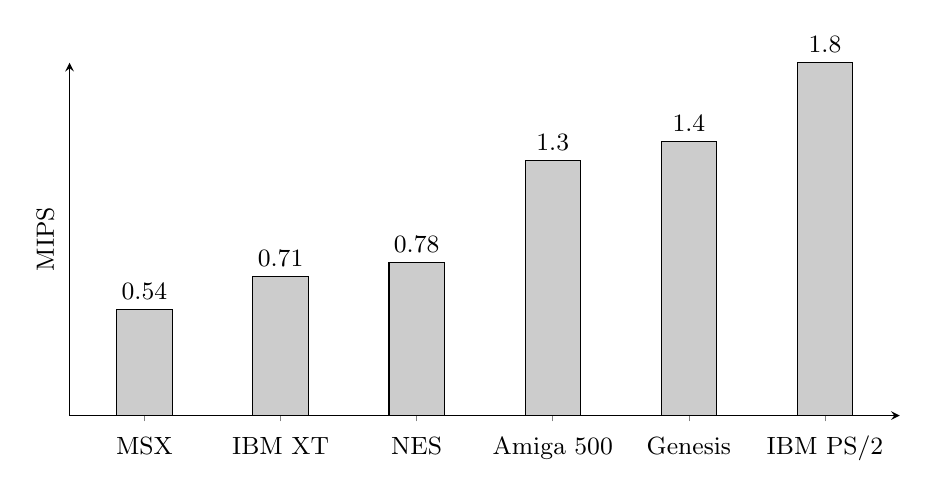
\begin{tikzpicture}[font=\small]
    \begin{axis}[
      width=\textwidth,
      height=0.5\textwidth,
      ybar=6pt,
      bar width=20pt,
      ylabel={MIPS},
      ymin=0,
      ytick=\empty,
      xtick=data,
      axis x line=bottom,
      axis y line=left,
      enlarge x limits=0.11,
      symbolic x coords={MSX, IBM XT, NES, Amiga 500, Genesis, IBM PS/2},
      xticklabel style={anchor=base,yshift=-\baselineskip},
      nodes near coords={\pgfmathprintnumber\pgfplotspointmeta}
    ]
      \addplot[fill=black!20,draw=black] coordinates {
        (MSX, 0.54)
        (IBM XT, 0.71)
        (NES, 0.78)
        (Amiga 500,1.3)
        (Genesis,1.4)
        (IBM PS/2, 1.8)
      };
    \end{axis}
   \end{tikzpicture}
   \caption{Consoles\protect\footnotemark vs PC, CPU comparison with MIPS\protect\footnotemark $^,$\protect\footnotemark.}
   \label{fig:ems_xms_layout}
 \end{figure}
 \addtocounter{footnote}{-2}
 \footnotetext{The MSX uses a Zilog Z80 running at 3.6MHz. The Amiga 500 and Genesis have a Motorola 68000 CPU respectively running at 7.16 MHz and 7.6 MHz. The NES uses a Ricoh 2A03 CPU running at 1.8 MHz.}
 \stepcounter{footnote}
 \footnotetext{Million Instructions Per Second.}
 \stepcounter{footnote}
 \footnotetext{Gamicus Fandom: https://gamicus.fandom.com/wiki/Instructions\_per\_second.}


Overall, it seemed impossible to create any reasonable side-scrolling game on the PC platform. But many around the world did not accept that and tinkered with the hardware to achieve unexpected results. Their ingenuity is what inspired me to write this book. \\

\par
I've chosen to divide this book into three chapters:
\begin{itemize}
  \item Chapter 2: The Hardware. An exploration of PC components from 1990.
  \item Chapter 3: The tools and assets. Which tools are used for game development and how are assets created and structured.
  \item Chapter 4: The Software. A deep dive into the Commander Keen game engine.

\end{itemize}

\par
By first showing the hardware constraints, I hope programmers will develop an appreciation for the software and how it navigated obstacles, sometimes turning limitations into advantages.\\

\par
This book focuses on \textit{Commander Keen in Keen Dreams}, which is developed after the first three releases in the series. The reason for this choice is straightforward: it is the only version with publicly released source code. Where relevant, I will also highlight technological differences across the versions of Commander Keen. However, code examples will be limited to Keen Dreams, due to the availability of the source material.\\

\begin{figure}[H]
  \centering
 \fbox{\includegraphics[width=1.0\textwidth]{screenshots_300dpi/Keen_Dreams.png}}
\caption{Commander Keen in Keen Dreams}
\end{figure}








\end{document}